\section{Deletesec}
\label{sec:Deletesec}
It is reasonable to start with two of the most intuitive and well known methods for classification, LDA and Logistic Regression. 
The point of this chapter is to give an introduction to classification through the use of these methods. They will only be considered in their most general form, and only with two classes. The term linear classifier refers to the fact that the decision boundary is linear in the features $\mathbf{x}$.
%
\section{LDA and Fisher's Linear Discriminant}
\label{sec:LDA and Fisher's Linear Discriminant}
LDA and Fisher's Linear Discriminant are in principle the same classifier. They only differ in the intuition behind the each method. Both will be showed in this section as they introduce different ways to approach a classification problem. The arguments are largely based on \cite{bishop} and \cite{modstat}, so no further references to these books will be made. 

\subsection{Fisher's Linear Discriminant}
\label{sub:Fisher's Linear Discriminant}
Fisher's Linear Discriminant try to find a discriminant hyperplane in the features $\mathbf{x}\in \mathbb{R}^D$. This is done by creating a vector $\mathbf{w}$, that the features are projected on, and thus reducing the problem to one dimension,
\begin{align}
  z = \mathbf{w}^T\mathbf{x}.
\end{align}
For a given $\mathbf{w}$,  a threshold $t$ can be chosen, and classification is done based on $z$'s relation to $t$.  I.e. classify to class $\mathcal{C}_1$ if $z > t$ and to class $\mathcal{C}_2$ if $z \leq t $. The problem is really therefore to find the vector $\mathbf{w}$ that gives the best class separation. One approach is to let $\mathbf{w}$ be proportional to the vector between the class means, i.e. $\mathbf{w} \propto (\bm{\mu}_2 - \bm{\mu}_1)$, where $\bm{\mu}_k = \sum_{i \in \mathcal{C}_k} \mathbf{x}_i/N_k$, and $N_k$ is the number of training points in $\mathcal{C}_k$. 
However, this does not take into account the orientation of the points around the mean, and is therefore often a bad choice. 
Fisher's approach was to take the \textit{within-class} variance into account. By minimize the variance of the groups' projections onto $\mathbf{w}$ ($s_k^2$ in \eqref{eq:fisherMax}), a better result could be obtained. So he want the $\mathbf{w}$ that maximize the between-class variance $(\mu_2 - \mu_1)^2$ and minimize the within-class variance $s_1^2 + s_2^2$, and suggested the following expression,
\begin{align}
  \label{eq:fisherMax} 
  \mathbf{w} &= \argmax_{\mathbf{v}} \frac{(\mu_2 - \mu_1)^2}{s_1^2 + s_2^2} \\
  s_k^2 &= \sum_{i \in \mathcal{C}_k} (z_i - \mu_k)^2, \quad \mu_k = \mathbf{v}^T\bm{\mu}_k.
\end{align}
Now let,
\begin{align}
  \mathbf{S}_W &= \mathbf{S}_1 + \mathbf{S}_2, \quad  \mathbf{S}_k =  \sum_{i \in \mathcal{C}_k} (\mathbf{x}_i - \bm{\mu}_k)(\mathbf{x}_i - \bm{\mu}_k)^T, \\
  \label{eq:SB} 
  \mathbf{S}_B &= (\bm{\mu}_2 - \bm{\mu}_1)(\bm{\mu}_2 - \bm{\mu}_1)^T,
\end{align}
denote the total within- and between-class covariances. \eqref{eq:fisherMax} can now be written as,
\begin{align}
  \mathbf{w} = \argmax_{\mathbf{v}}  \frac{\mathbf{v}^T\mathbf{S}_B \mathbf{v}}{\mathbf{v}^T \mathbf{S}_W \mathbf{v}}.
\end{align}
By differentiating and setting the expression equal to zero yields,
\begin{align}
  \label{eq:optfish} 
  (\mathbf{w}^T \mathbf{S}_B \mathbf{w})\mathbf{S}_W \mathbf{w} = (\mathbf{w}^T \mathbf{S}_W \mathbf{w})\mathbf{S}_B \mathbf{w}.
\end{align}
From \eqref{eq:SB}, it follows that that $(\bm{\mu}_2 - \bm{\mu}_1)$ is proportional to $\mathbf{S}_B \mathbf{w}$. Dropping the constants in \eqref{eq:optfish}, this yields Fisher's linear discriminant,
\begin{align}
  \mathbf{w} \propto \mathbf{S}_W^{-1} (\bm \mu_2 - \bm \mu_1).
\end{align}
Note that even though the terms \textit{variance} and \textit{covariance} are used, the expressions are not averaged. This is just to simplify notation. 
\\
\\
\subsection{LDA}
\label{sub:LDA}
Before LDA is explained, it is useful to make the goal of classification more explicit. One way is through defining the \textit{expected prediction error}, $\mathrm{EPE}$.
Let $ C(\mathbf{x})$ be a classifier, and $L$ the loss function the method tries to minimize. As mentioned in the introduction, only $0/1$ loss will be considered here, and $L$ takes the form,
\begin{align}
  L(y, C(\mathbf{x})) = I\{ C(\mathbf{x}) \neq y \}. 
\end{align}
The expected prediction error is then defined as,
\begin{align}
  \mathrm{EPE}(C(\mathbf{x})) 
  &= \E_{\mathbf{x}, y}[L(y, C(\mathbf{x}))] = \E_{\mathbf{x}}[\E_{y}[L(y, C(\mathbf{x})) \mid  \mathbf{x}]].
\end{align}
The goal of a classifier should be to minimize this function.
\begin{align}
  C^*(\mathbf{x}) 
  &= \argmin_{ C} \mathrm{EPE}(C(\mathbf{x})) = \argmin_{ C} \E_{y}[L(y,  C(\mathbf{x})) \mid  \mathbf{x}] \notag \\
  &= \argmin_{ C} \E_{y}[I\{ C(\mathbf{x}) \neq y \} \mid  \mathbf{x}] \notag \\
  \label{eq:EPE} 
  &= \argmax_{ C} P_{y}\left( C(\mathbf{x}) = y  \mid  \mathbf{x}  \right) = \E_y [y \mid  \mathbf{x}].
\end{align}
Thus, a framework for classification has been established in form of either an optimization problem, or a conditional expectation.
\\
\\
The derivation for LDA takes a Bayesian approach. 
Assume knowledge of a prior distributions for the classes $P(y = k) = \pi_k$, and conditional distributions for $\mathbf{x}$ given $y$, $f_k(\mathbf{x})$. Simple application of the Bayes theorem yields,
\begin{align}
  P(y=k\mid \mathbf{x}) = \frac{f_k(\mathbf{x}) \pi_k}{\sum^{K}_{i=1} f_i(\mathbf{x})\pi_i} .
\end{align}
Using this posterior distribution, a classifier can be constructed from \eqref{eq:EPE},
\begin{align}
  \label{eq:bayesian} 
  C(\mathbf{x}) = \argmax_k P(y=k\mid \mathbf{x}).
\end{align}
The literature often refers to this as the \textit{Bayes classifier} \cite{modstat}. As it is the best on can do under 0/1 loss, it is often used as a benchmark in simulation studies. 

LDA assumes the conditional distributions are multivariate Gaussian with equal covariance $\bm{\Sigma}$ and individual means $\bm\mu_k$,
\begin{align}
  f_k(\mathbf{x}) =  \frac{1}{(2\pi)^{N_k/2}\mid \bm{\Sigma}\mid ^{1/2}} \exp\left( -\frac{1}{2} (\mathbf{x}-\bm \mu_k)^T \bm{\Sigma}^{-1} (\mathbf{x}-\bm \mu_k)\right).
\end{align}
The classifier in \eqref{eq:bayesian} can now be constructed by evaluating the log-ratio of the probabilities,
\begin{align}
  \label{eq:lda} 
  \log{\frac{P(y=2\mid \mathbf{x})}{P(y=1\mid \mathbf{x})}} &= \log{\frac{f_2(\mathbf{x})}{f_1(\mathbf{x})} } + \log{\frac{\pi_2}{\pi_1} } \notag \ \\
  &= \log{\frac{\pi_2}{\pi_1}} -\frac{1}{2} (\bm \mu_2+\bm \mu_1)^T \bm{\Sigma}^{-1} (\bm \mu_2-\bm \mu_1) \\
  & \quad + \mathbf{x}^T\bm{\Sigma}^{-1} (\bm \mu_2-\bm \mu_1).
  \notag \ 
\end{align}
So one classify to $\mathcal{C}_2$ if \eqref{eq:lda} is positive and to $\mathcal{C}_1$ if not. 

Another approach is to use only the last part of \eqref{eq:lda}, $\mathbf{x}^T\bm{\Sigma}^{-1} (\bm \mu_1-\bm \mu_2)$, and classify based on some threshold $t$ found by e.g. cross-validation (see Appendix~\ref{sec:Cross-validation}). This might be a good idea when the Gaussian assumptions are wrong. Cross-validation is not dependent on any distribution, and can give a better threshold. 
\\
\\
When using LDA, the parameters are not know, so they are usually estimated from the training data by,
\begin{align}
   \hat{\pi}_k &= \frac{N_k}{N},  \\
   \hat{\bm \mu}_k &= \frac{1}{N_k} \sum_{i \in \mathcal{C}_k}\mathbf{x}_i, \\
   \hat{\bm \Sigma} &= \frac{1}{N-2} \sum_{k = 1}^{2} \sum_{i \in \mathcal{C}_k}(\mathbf{x}_i - \hat{\bm{\mu}}_k)(\mathbf{x}_i - \hat{\bm{\mu}}_k)^T.
\end{align}
It now becomes clear that both LDA and Fisher's linear discriminant do the same projection. The only difference between the methods is that because of the Gaussian assumptions, LDA can give a suggested threshold.
%
\section{Logistic Regression}
\label{sec:Logistic Regression}
The goal of Logistic Regression is to model the posterior class-probabilities and create a classifier based on them. As the probabilities should sum to one, it is obvious that they can not be linear in $\mathbf{x}$. Instead the log odds are assumed to be linear in $\mathbf{x}$,
\begin{align}
  \label{eq:logclass} 
   \log \frac{P(y=2\mid \mathbf{x})}{P(y=1\mid \mathbf{x})} = \beta_0 + \mathbf{x}^T\bm \beta.
\end{align}
From here on notation is simplified by writing $\beta_0 + \mathbf{x}^T \bm \beta$ as $\mathbf{x}^T \bm \beta$.
The function,
\begin{align}
  logit(p_{ki}) = \log  \frac{p_{ki}}{1-p_{ki}},
\end{align}
where $p_{ki} = P(y=k\mid \mathbf{x_i})$, is called the \textit{logit function} or \textit{logit link}. By inverting the logit function it becomes clear that the posterior probabilities sum to \textit{one},
\begin{align}
  p_{2i} &=  \frac{e^{\mathbf{x}_i^T\bm \beta}}{1 + e^{\mathbf{x}_i^T\bm \beta}}, \\
  p_{1i} &=  \frac{1}{1 + e^{\mathbf{x}_i^T\bm \beta}}.
\end{align}
There are other possible choices than the logit function, e.g. the probit function based on Gaussian assumptions. They will however not be covered in this report. 
The logit link is not necessarily used because it is a good assumption. Often it is used as no better assumptions are made.

To find good values for $\bm \beta$, it is common to use the Maximum likelihood estimator, or MLE. Let $n_i$ be the number of training samples in group $i$. A group in this sense is data points with the same covariates $\mathbf{x}_i = \mathbf{x}_j$. Let $Z_i$ the number of points in group $i$ that has class $2$. This means $Z_i$ is binomially distributed,
\begin{align}
  P(Z_i = z_i) = \binom{n_i}{z_i} p_{2i}^{z_i} (1-p_{2i})^{n_i - z_i}.
\end{align}
So the likelihood and log-likelihood are,
\begin{align}
  L(\beta) &= \prod_{i = 1}^{N} P(Z_i = z_i). \\
  l(\beta) &\propto \sum^{N}_{i=1} z_i \log p_{2i} + (n_i - z_i) \log (1- p_{2i}).
\end{align}
There is no analytical solution that maximizes the likelihood, so one has to use a numerical optimization algorithm to find the MLE.  

After $\bm \beta$ is found, one can create a classifier the same way as for LDA, i.e. classify to $\mathcal{C}_2$ if \eqref{eq:logclass} is positive and to $\mathcal{C}_1$ if not. However, this assumes the logit link gives accurate probabilities. Often the choice of logit link is based on lack of a better choice so there is little suggesting the probabilities are particularly accurate. It might therefore be better to classify based on a threshold found by e.g. cross-validation.
%
\section{Comparing LDA and Logistic Regression}
\label{sub:LDA and Logistic Regre}
<<ldaVsLogistic, echo = FALSE>>=
source("../code/ldaVsLogistic.R")
@
Comparing LDA and logistic regression, it is clear that they are both linear in the log odds. Obviously this does not restrict the decision boundary to be linear in $x_1, x_2, \ldots , x_D$. Polynomial terms and interaction terms can be used, e.g. $x_1, x_2, x_1^2, x_1 x_2$, allowing a pretty flexible decision boundary. Both methods are also easy to generalize to multiclass classifiers, but this will not be covered here. 
\\
\\
To compare the two methods performance a toy example was generated by drawing \Sexpr{N} training points from each of two classes. The points were drawn from a multivariate normal distribution in \Sexpr{D} dimensions, both with the same covariance, but with different means. The draws are displayed in Figure~\ref{fig:ldaVsLogistic}. LDA and Logistic Regression was fitted to the data set using the R functions \verb+lda+ from the \verb+MASS+ package \citep{mass} and \verb+glm+ from the \verb+stats+ package \citep{stats}. In the figure, the default decision boundaries was plotted, along with the optimal decision boundary.

Obviously, the experiment was in great favor to LDA as it was constructed based on the assumptions used in LDA, but from the plot, there is little that separates the two solutions. They are both very close to the optimal solution.

A test set was also generated using \Sexpr{Ntest} realizations from each group. The two methods performed almost the same. LDA had a misclassification error of \Sexpr{mceLda}, and logistic regression had \Sexpr{mceLog}. This is pretty close to the optimal MCE of \ldots \todo{Optimal MCE} \\
\\
%
\begin{figure}[h!]
\begin{center}
    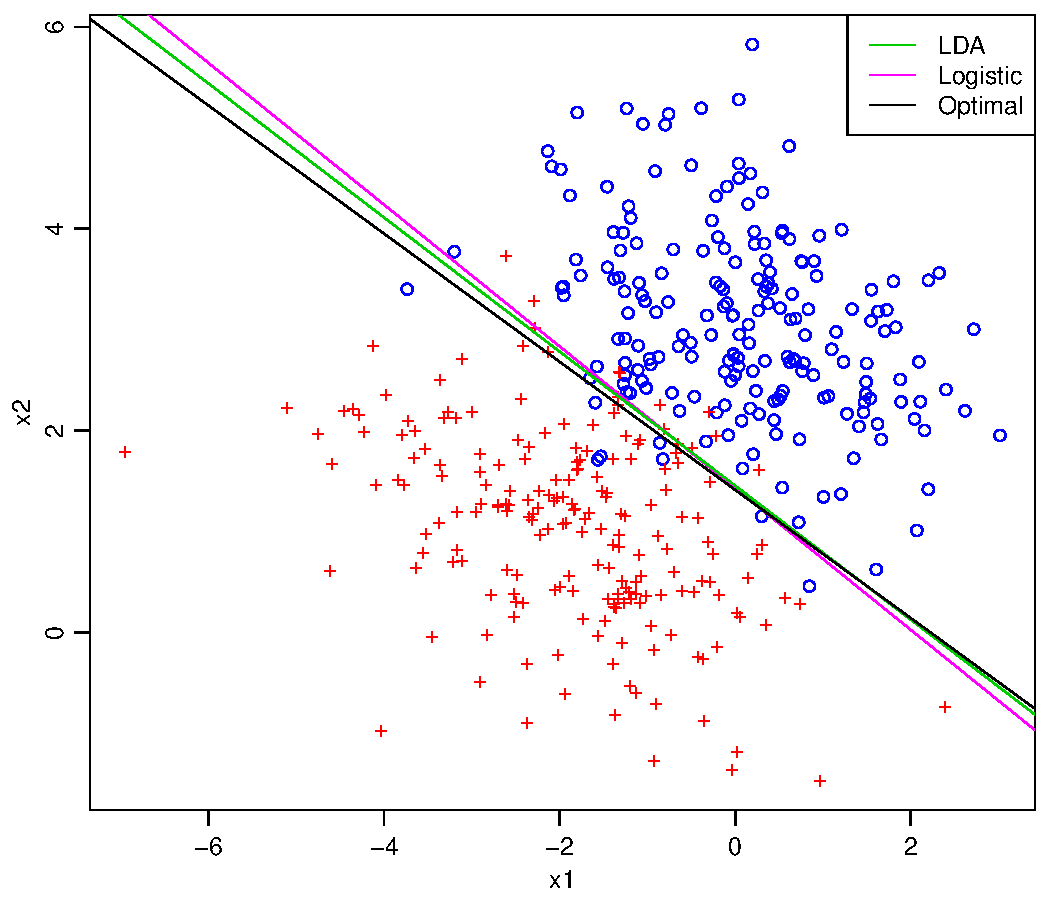
\includegraphics[scale=0.5]{./figures/ldaVsLogistic.pdf}
\end{center}
\caption{Decision boundaries for the two classes, each of size \Sexpr{N}, drawn from multigaussians with same covariance and different means.}
\label{fig:ldaVsLogistic}
\end{figure}
\\
Although, the methods seem very similar, and in the toy example had almost equal performance, their can perform very different. LDA is based on more specific assumptions than Logistic Regression. In the derivation of Fisher's Linear Discriminant, it was clear that LDA has applications outside the Gaussian assumptions. Nevertheless, today it is not considered a particular good method. Logistic Regression, on the other hand, is still widely used.  In fact, by penalizing $\bm \beta$ in the log-likelihood function, it can be quite powerful (see \cite{modstat}).
